\documentclass[../main/NEMO_manual]{subfiles}

\begin{document}

\chapter{Model Basics}
\label{chap:MB}

\chaptertoc

\paragraph{Changes record} ~\\

{\footnotesize
  \begin{tabular}{l||l|l}
    Release          & Author(s)                                   & Modifications       \\
    \hline
    {\em        4.0} & {\em Mike Bell                            } & {\em Review       } \\
    {\em        3.6} & {\em Tim Graham and Gurvan Madec          } & {\em Updates      } \\
    {\em $\leq$ 3.4} & {\em Gurvan Madec and S\'{e}bastien Masson} & {\em First version} \\
  \end{tabular}
}

\clearpage

%% =================================================================================================
\section{Primitive equations}
\label{sec:MB_PE}

%% =================================================================================================
\subsection{Vector invariant formulation}
\label{subsec:MB_PE_vector}

The ocean is a fluid that can be described to a good approximation by the primitive equations,
\ie\ the Navier-Stokes equations along with a nonlinear equation of state which
couples the two active tracers (temperature and salinity) to the fluid velocity,
plus the following additional assumptions made from scale considerations:

\begin{labeling}{Neglect of additional Coriolis terms}
\item [\textit{Spherical Earth approximation}] The geopotential surfaces are assumed to
  be oblate spheroids that follow the Earth's bulge;
  these spheroids are approximated by spheres with gravity locally vertical
  (parallel to the Earth's radius) and independent of latitude
  \citep[][section 2]{white.hoskins.ea_QJRMS05}.
\item [\textit{Thin-shell approximation}] The ocean depth is neglected compared to the earth's radius
\item [\textit{Turbulent closure hypothesis}] The turbulent fluxes
  (which represent the effect of small scale processes on the large-scale)
  are expressed in terms of large-scale features
\item [\textit{Boussinesq hypothesis}] Density variations are neglected except in
  their contribution to the buoyancy force
  \begin{equation}
    \label{eq:MB_PE_eos}
    \rho = \rho \ (T,S,p)
  \end{equation}
\item [\textit{Hydrostatic hypothesis}] The vertical momentum equation is reduced to
  a balance between the vertical pressure gradient and the buoyancy force
  (this removes convective processes from the initial Navier-Stokes equations and so
  convective processes must be parameterized instead)
  \begin{equation}
    \label{eq:MB_PE_hydrostatic}
    \pd[p]{z} = - \rho \ g
  \end{equation}
\item [\textit{Incompressibility hypothesis}] The three dimensional divergence of
  the velocity vector $\vect U$ is assumed to be zero.
  \begin{equation}
    \label{eq:MB_PE_continuity}
    \nabla \cdot \vect U = 0
  \end{equation}
\item [\textit{Neglect of additional Coriolis terms}] The Coriolis terms that vary with
  the cosine of latitude are neglected.
  These terms may be non-negligible where the Brunt-V\"{a}is\"{a}l\"{a} frequency $N$ is small,
  either in the deep ocean or in the sub-mesoscale motions of the mixed layer,
  or near the equator \citep[][section 1]{white.hoskins.ea_QJRMS05}.
  They can be consistently included as part of the ocean dynamics
  \citep[][section 3(d)]{white.hoskins.ea_QJRMS05} and are retained in the MIT ocean model.
\end{labeling}

Because the gravitational force is so dominant in the equations of large-scale motions,
it is useful to choose an orthogonal set of unit vectors $(i,j,k)$ linked to the Earth such that
$k$ is the local upward vector and $(i,j)$ are two vectors orthogonal to $k$,
\ie\ tangent to the geopotential surfaces.
Let us define the following variables:
$\vect U$ the vector velocity, $\vect U = \vect U_h + w \, \vect k$
(the subscript $h$ denotes the local horizontal vector, \ie\ over the $(i,j)$ plane),
$T$ the potential temperature, $S$ the salinity, $\rho$ the \textit{in situ} density.
The vector invariant form of the primitive equations in the $(i,j,k)$ vector system provides
the following equations:
\begin{subequations}
  \label{eq:MB_PE}
  \begin{gather}
    \shortintertext{$-$ the momentum balance}
    \label{eq:MB_PE_dyn}
    \pd[\vect U_h]{t} = - \lt[ (\nabla \times \vect U) \times \vect U + \frac{1}{2} \nabla \lt( \vect U^2 \rt) \rt]_h - f \; k \times \vect U_h - \frac{1}{\rho_o} \nabla_h p + \vect D^{\vect U} + \vect F^{\vect U}
    \shortintertext{$-$ the heat and salt conservation equations}
    \label{eq:MB_PE_tra_T}
    \pd[T]{t} = - \nabla \cdot (T \ \vect U) + D^T + F^T \\
    \label{eq:MB_PE_tra_S}
    \pd[S]{t} = - \nabla \cdot (S \ \vect U) + D^S + F^S
  \end{gather}
\end{subequations}
where $\nabla$ is the generalised derivative vector operator in $(i,j,k)$ directions, $t$ is the time,
$z$ is the vertical coordinate, $\rho$ is the \textit{in situ} density given by the equation of state
(\autoref{eq:MB_PE_eos}), $\rho_o$ is a reference density, $p$ the pressure,
$f = 2 \vect \Omega \cdot k$ is the Coriolis acceleration
(where $\vect \Omega$ is the Earth's angular velocity vector),
and $g$ is the gravitational acceleration.
$\vect D^{\vect U}$, $D^T$ and $D^S$ are the parameterisations of small-scale physics for momentum,
temperature and salinity, and $\vect F^{\vect U}$, $F^T$ and $F^S$ surface forcing terms.
Their nature and formulation are discussed in \autoref{sec:MB_zdf_ldf} and
\autoref{subsec:MB_boundary_condition}.

%% =================================================================================================
\subsection{Boundary conditions}
\label{subsec:MB_boundary_condition}

An ocean is bounded by complex coastlines, bottom topography at its base and
an air-sea or ice-sea interface at its top.
These boundaries can be defined by two surfaces, $z = - H(i,j)$ and $z = \eta(i,j,k,t)$,
where $H$ is the depth of the ocean bottom and $\eta$ is the height of the sea surface
(discretisation can introduce additional artificial ``side-wall'' boundaries).
Both $H$ and $\eta$ are referenced to a surface of constant geopotential
(\ie\ a mean sea surface height) on which $z = 0$ (\autoref{fig:MB_ocean_bc}).
Through these two boundaries, the ocean can exchange fluxes of heat, fresh water, salt,
and momentum with the solid earth, the continental margins, the sea ice and the atmosphere.
However, some of these fluxes are so weak that
even on climatic time scales of thousands of years they can be neglected.
In the following, we briefly review the fluxes exchanged at the interfaces between the ocean and
the other components of the earth system.

\begin{figure}
  \centering
  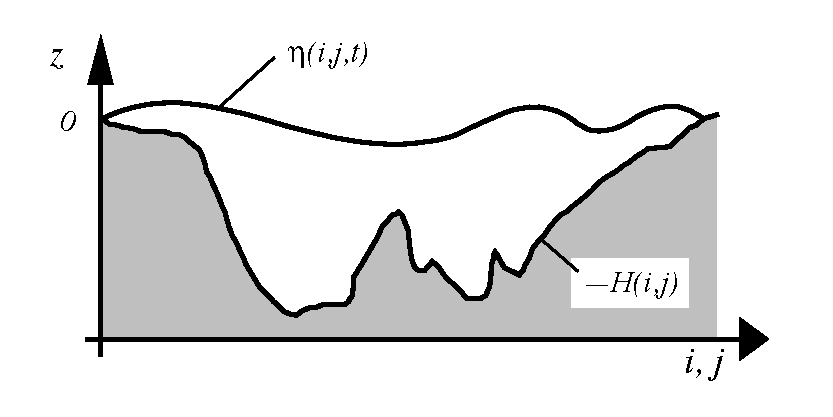
\includegraphics[width=0.66\textwidth]{MB_ocean_bc}
  \caption[Ocean boundary conditions]{
    The ocean is bounded by two surfaces, $z = - H(i,j)$ and $z = \eta(i,j,t)$,
    where $H$ is the depth of the sea floor and $\eta$ the height of the sea surface.
    Both $H$ and $\eta$ are referenced to $z = 0$.}
  \label{fig:MB_ocean_bc}
\end{figure}

\begin{description}
\item [Land - ocean] The major flux between continental margins and the ocean is a mass exchange of
  fresh water through river runoff.
  Such an exchange modifies the sea surface salinity especially in the vicinity of major river mouths.
  It can be neglected for short range integrations but
  has to be taken into account for long term integrations as
  it influences the characteristics of water masses formed (especially at high latitudes).
  It is required in order to close the water cycle of the climate system.
  It is usually specified as a fresh water flux at the air-sea interface in
  the vicinity of river mouths.
\item [Solid earth - ocean] Heat and salt fluxes through the sea floor are small,
  except in special areas of little extent.
  They are usually neglected in the model \footnote{
    In fact, it has been shown that the heat flux associated with the solid Earth cooling
    (\ie\ the geothermal heating) is not negligible for
    the thermohaline circulation of the world ocean (see \autoref{subsec:TRA_bbc}).
  }.
  The boundary condition is thus set to no flux of heat and salt across solid boundaries.
  For momentum, the situation is different.
  There is no flow across solid boundaries,
  \ie\ the velocity normal to the ocean bottom and coastlines is zero
  (in other words, the bottom velocity is parallel to solid boundaries).
  This kinematic boundary condition can be expressed as:
  \begin{equation}
    \label{eq:MB_w_bbc}
    w = - \vect U_h \cdot \nabla_h (H)
  \end{equation}
  In addition, the ocean exchanges momentum with the earth through frictional processes.
  Such momentum transfer occurs at small scales in a boundary layer.
  It must be parameterized in terms of turbulent fluxes using
  bottom and/or lateral boundary conditions.
  Its specification depends on the nature of the physical parameterisation used for
  $\vect D^{\vect U}$ in \autoref{eq:MB_PE_dyn}.
  It is discussed in \autoref{eq:MB_zdf}. % and Chap. III.6 to 9.
\item [Atmosphere - ocean] The kinematic surface condition plus the mass flux of fresh water PE
  (the precipitation minus evaporation budget) leads to:
  \[
    % \label{eq:MB_w_sbc}
    w = \pd[\eta]{t} + \lt. \vect U_h \rt|_{z = \eta} \cdot \nabla_h (\eta) + P - E
  \]
  The dynamic boundary condition, neglecting the surface tension
  (which removes capillary waves from the system) leads to
  the continuity of pressure across the interface $z = \eta$.
  The atmosphere and ocean also exchange horizontal momentum (wind stress), and heat.
\item [Sea ice - ocean] The ocean and sea ice exchange heat, salt, fresh water and momentum.
  The sea surface temperature is constrained to be at the freezing point at the interface.
  Sea ice salinity is very low ($\sim4-6 \, psu$) compared to those of the ocean ($\sim34 \, psu$).
  The cycle of freezing/melting is associated with fresh water and salt fluxes that
  cannot be neglected.
\end{description}

%% =================================================================================================
\section{Horizontal pressure gradient}
\label{sec:MB_hor_pg}

%% =================================================================================================
\subsection{Pressure formulation}
\label{subsec:MB_p_formulation}

The total pressure at a given depth $z$ is composed of a surface pressure $p_s$ at
a reference geopotential surface ($z = 0$) and a hydrostatic pressure $p_h$ such that:
$p(i,j,k,t) = p_s(i,j,t) + p_h(i,j,k,t)$.
The latter is computed by integrating (\autoref{eq:MB_PE_hydrostatic}),
assuming that pressure in decibars can be approximated by depth in meters in (\autoref{eq:MB_PE_eos}).
The hydrostatic pressure is then given by:
\[
  % \label{eq:MB_pressure}
  p_h (i,j,z,t) = \int_{\varsigma = z}^{\varsigma = 0} g \; \rho (T,S,\varsigma) \; d \varsigma
\]
Two strategies can be considered for the surface pressure term:
\begin{enumerate*}[label=(\textit{\alph*})]
\item introduce of a new variable $\eta$, the free-surface elevation,
for which a prognostic equation can be established and solved;
\item assume that the ocean surface is a rigid lid,
on which the pressure (or its horizontal gradient) can be diagnosed.
\end{enumerate*}
When the former strategy is used, one solution of the free-surface elevation consists of
the excitation of external gravity waves.
The flow is barotropic and the surface moves up and down with gravity as the restoring force.
The phase speed of such waves is high (some hundreds of metres per second) so that
the time step has to be very short when they are present in the model.
The latter strategy filters out these waves since the rigid lid approximation implies $\eta = 0$,
\ie\ the sea surface is the surface $z = 0$.
This well known approximation increases the surface wave speed to infinity and
modifies certain other longwave dynamics (\eg\ barotropic Rossby or planetary waves).
The rigid-lid hypothesis is an obsolescent feature in modern OGCMs.
It has been available until the release 3.1 of \NEMO,
and it has been removed in release 3.2 and followings.
Only the free surface formulation is now described in this document (see the next sub-section).

%% =================================================================================================
\subsection{Free surface formulation}
\label{subsec:MB_free_surface}

In the free surface formulation, a variable $\eta$, the sea-surface height,
is introduced which describes the shape of the air-sea interface.
This variable is solution of a prognostic equation which is established by
forming the vertical average of the kinematic surface condition (\autoref{eq:MB_w_bbc}):
\begin{equation}
  \label{eq:MB_ssh}
  \pd[\eta]{t} = - D + P - E \quad \text{where} \quad D = \nabla \cdot \lt[ (H + \eta) \; \overline{U}_h \, \rt]
\end{equation}
and using (\autoref{eq:MB_PE_hydrostatic}) the surface pressure is given by:
$p_s = \rho \, g \, \eta$.

Allowing the air-sea interface to move introduces
the \textbf{E}xternal \textbf{G}ravity \textbf{W}aves (EGWs) as
a class of solution of the primitive equations.
These waves are barotropic (\ie\ nearly independent of depth) and their phase speed is quite high.
Their time scale is short with respect to the other processes described by the primitive equations.

Two choices can be made regarding the implementation of the free surface in the model,
depending on the physical processes of interest.
\begin{itemize}
\item If one is interested in EGWs, in particular the tides and their interaction with
  the baroclinic structure of the ocean (internal waves) possibly in shallow seas,
  then a non linear free surface is the most appropriate.
  This means that no approximation is made in \autoref{eq:MB_ssh} and that
  the variation of the ocean volume is fully taken into account.
  Note that in order to study the fast time scales associated with EGWs it is necessary to
  minimize time filtering effects
  (use an explicit time scheme with very small time step,
  or a split-explicit scheme with reasonably small time step,
  see \autoref{subsec:DYN_spg_exp} or \autoref{subsec:DYN_spg_ts}).
\item If one is not interested in EGWs but rather sees them as high frequency noise,
  it is possible to apply an explicit filter to slow down the fastest waves while
  not altering the slow barotropic Rossby waves.
  If further, an approximative conservation of heat and salt contents is sufficient for
  the problem solved, then it is sufficient to solve a linearized version of \autoref{eq:MB_ssh},
  which still allows to take into account freshwater fluxes applied at the ocean surface
  \citep{roullet.madec_JGR00}.
  Nevertheless, with the linearization, an exact conservation of heat and salt contents is lost.
\end{itemize}
The filtering of EGWs in models with a free surface is usually
a matter of discretisation of the temporal derivatives,
using a split-explicit method \citep{killworth.webb.ea_JPO91, zhang.endoh_JGR92} or
the implicit scheme \citep{dukowicz.smith_JGR94} or the addition of a filtering force in
the momentum equation \citep{roullet.madec_JGR00}.
With the present release, \NEMO\ offers the choice between an explicit free surface
(see \autoref{subsec:DYN_spg_exp}) or a split-explicit scheme strongly inspired the one proposed by
\citet{shchepetkin.mcwilliams_OM05} (see \autoref{subsec:DYN_spg_ts}).

%% =================================================================================================
\section{Curvilinear \textit{z}-coordinate system}
\label{sec:MB_zco}

%% =================================================================================================
\subsection{Tensorial formalism}
\label{subsec:MB_tensorial}

In many ocean circulation problems, the flow field has regions of enhanced dynamics
(\ie\ surface layers, western boundary currents, equatorial currents, or ocean fronts).
The representation of such dynamical processes can be improved by
specifically increasing the model resolution in these regions.
As well, it may be convenient to use a lateral boundary-following coordinate system to
better represent coastal dynamics.
Moreover, the common geographical coordinate system has a singular point at the North Pole that
cannot be easily treated in a global model without filtering.
A solution consists of introducing an appropriate coordinate transformation that
shifts the singular point onto land \citep{madec.imbard_CD96, murray_JCP96}.
As a consequence,
it is important to solve the primitive equations in various curvilinear coordinate systems.
An efficient way of introducing an appropriate coordinate transform can be found when
using a tensorial formalism.
This formalism is suited to any multidimensional curvilinear coordinate system.
Ocean modellers mainly use three-dimensional orthogonal grids on the sphere
(spherical earth approximation), with preservation of the local vertical.
Here we give the simplified equations for this particular case.
The general case is detailed by \citet{eiseman.stone_SR80} in
their survey of the conservation laws of fluid dynamics.

Let $(i,j,k)$ be a set of orthogonal curvilinear coordinates on
the sphere associated with the positively oriented orthogonal set of unit vectors
$(i,j,k)$ linked to the earth such that
$k$ is the local upward vector and $(i,j)$ are two vectors orthogonal to $k$,
\ie\ along geopotential surfaces (\autoref{fig:MB_referential}).
Let $(\lambda,\varphi,z)$ be the geographical coordinate system in which a position is defined by
the latitude $\varphi(i,j)$, the longitude $\lambda(i,j)$ and
the distance from the centre of the earth $a + z(k)$ where $a$ is the earth's radius and
$z$ the altitude above a reference sea level (\autoref{fig:MB_referential}).
The local deformation of the curvilinear coordinate system is given by $e_1$, $e_2$ and $e_3$,
the three scale factors:
\begin{equation}
  \label{eq:MB_scale_factors}
    e_1 = (a + z) \lt[ \lt( \pd[\lambda]{i} \cos \varphi \rt)^2 + \lt( \pd[\varphi]{i} \rt)^2 \rt]^{1/2} \quad e_2 = (a + z) \lt[ \lt( \pd[\lambda]{j} \cos \varphi \rt)^2 + \lt( \pd[\varphi]{j} \rt)^2 \rt]^{1/2} \quad e_3 = \lt( \pd[z]{k} \rt)
\end{equation}

\begin{figure}
  \centering
  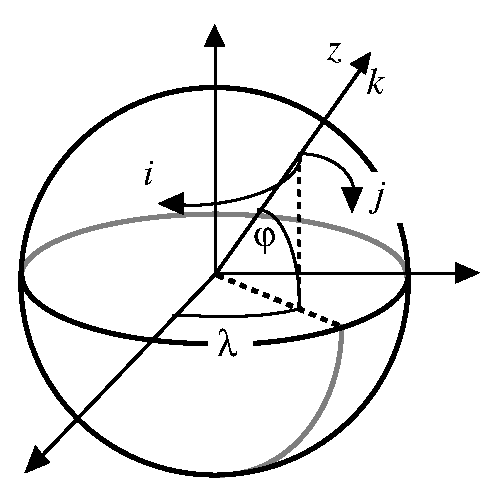
\includegraphics[width=0.33\textwidth]{MB_earth_referential}
  \caption[Geographical and curvilinear coordinate systems]{
    the geographical coordinate system $(\lambda,\varphi,z)$ and the curvilinear
    coordinate system $(i,j,k)$.}
  \label{fig:MB_referential}
\end{figure}

Since the ocean depth is far smaller than the earth's radius, $a + z$, can be replaced by $a$ in
(\autoref{eq:MB_scale_factors}) (thin-shell approximation).
The resulting horizontal scale factors $e_1$, $e_2$  are independent of $k$ while
the vertical scale factor is a single function of $k$ as $k$ is parallel to $z$.
The scalar and vector operators that appear in the primitive equations
(\autoref{eq:MB_PE_dyn} to \autoref{eq:MB_PE_eos}) can then be written in the tensorial form,
invariant in any orthogonal horizontal curvilinear coordinate system transformation:
\begin{subequations}
  % \label{eq:MB_discrete_operators}
  \begin{align}
    \label{eq:MB_grad}
    \nabla q &=   \frac{1}{e_1} \pd[q]{i} \; \vect i + \frac{1}{e_2} \pd[q]{j} \; \vect j + \frac{1}{e_3} \pd[q]{k} \; \vect k \\
    \label{eq:MB_div}
    \nabla \cdot \vect A &=   \frac{1}{e_1 \; e_2} \lt[ \pd[(e_2 \; a_1)]{\partial i} + \pd[(e_1 \; a_2)]{j} \rt] + \frac{1}{e_3} \lt[ \pd[a_3]{k} \rt] \\
    \label{eq:MB_curl}
      \nabla \times \vect{A} &=   \lt[ \frac{1}{e_2} \pd[a_3]{j} - \frac{1}{e_3} \pd[a_2]{k}   \rt] \vect i + \lt[ \frac{1}{e_3} \pd[a_1]{k} - \frac{1}{e_1} \pd[a_3]{i}   \rt] \vect j + \frac{1}{e_1 e_2} \lt[ \pd[(e_2 a_2)]{i} - \pd[(e_1 a_1)]{j} \rt] \vect k \\
    \label{eq:MB_lap}
    \Delta q &= \nabla \cdot (\nabla q) \\
    \label{eq:MB_lap_vector}
    \Delta \vect A &= \nabla (\nabla \cdot \vect A) - \nabla \times (\nabla \times \vect A)
  \end{align}
\end{subequations}
where $q$ is a scalar quantity and
$\vect A = (a_1,a_2,a_3)$ a vector in the $(i,j,k)$ coordinates system.

%% =================================================================================================
\subsection{Continuous model equations}
\label{subsec:MB_zco_Eq}

In order to express the Primitive Equations in tensorial formalism,
it is necessary to compute the horizontal component of the non-linear and viscous terms of
the equation using \autoref{eq:MB_grad}) to \autoref{eq:MB_lap_vector}.
Let us set $\vect U = (u,v,w) = \vect U_h + w \; \vect k $,
the velocity in the $(i,j,k)$ coordinates system,
and define the relative vorticity $\zeta$ and the divergence of the horizontal velocity field $\chi$,
by:
\begin{gather}
  \label{eq:MB_curl_Uh}
  \zeta = \frac{1}{e_1 e_2} \lt[ \pd[(e_2 \, v)]{i} - \pd[(e_1 \, u)]{j} \rt] \\
  \label{eq:MB_div_Uh}
  \chi  = \frac{1}{e_1 e_2} \lt[ \pd[(e_2 \, u)]{i} + \pd[(e_1 \, v)]{j} \rt]
\end{gather}

Using again the fact that the horizontal scale factors $e_1$ and $e_2$ are independent of $k$ and that
$e_3$  is a function of the single variable $k$,
$NLT$ the nonlinear term of \autoref{eq:MB_PE_dyn} can be transformed as follows:
\begin{align*}
  NLT &= \lt[ (\nabla \times {\vect U}) \times {\vect U} + \frac{1}{2} \nabla \lt( {\vect U}^2 \rt) \rt]_h \\
      &= \lt(
        \begin{array}{*{20}c}
          \lt[ \frac{1}{e_3} \pd[u]{k} - \frac{1}{e_1} \pd[w]{i} \rt] w - \zeta \; v   \\
          \zeta \; u - \lt[ \frac{1}{e_2} \pd[w]{j} - \frac{1}{e_3} \pd[v]{k} \rt] \ w
        \end{array}
  \rt)
  + \frac{1}{2} \lt(
  \begin{array}{*{20}c}
    \frac{1}{e_1} \pd[(u^2 + v^2 + w^2)]{i} \\
    \frac{1}{e_2} \pd[(u^2 + v^2 + w^2)]{j}
  \end{array}
  \rt) \\
      &= \lt(
        \begin{array}{*{20}c}
          -\zeta \; v \\
          \zeta \; u
        \end{array}
  \rt)
  + \frac{1}{2} \lt(
  \begin{array}{*{20}c}
    \frac{1}{e_1} \pd[(u^2 + v^2)]{i} \\
    \frac{1}{e_2} \pd[(u^2 + v^2)]{j}
  \end{array}
  \rt)
  + \frac{1}{e_3} \lt(
  \begin{array}{*{20}c}
    w \; \pd[u]{k} \\
    w \; \pd[v]{k}
  \end{array}
  \rt)
  - \lt(
  \begin{array}{*{20}c}
    \frac{w}{e_1} \pd[w]{i} - \frac{1}{2 e_1} \pd[w^2]{i} \\
    \frac{w}{e_2} \pd[w]{j} - \frac{1}{2 e_2} \pd[w^2]{j}
  \end{array}
  \rt)
\end{align*}
The last term of the right hand side is obviously zero,
and thus the \textbf{N}on\textbf{L}inear \textbf{T}erm ($NLT$) of \autoref{eq:MB_PE_dyn} is written in
the $(i,j,k)$ coordinate system:
\begin{equation}
  \label{eq:MB_vector_form}
  NLT = \zeta \; \vect k \times \vect U_h + \frac{1}{2} \nabla_h \lt( \vect U_h^2 \rt) + \frac{1}{e_3} w \pd[\vect U_h]{k}
\end{equation}

This is the so-called \textit{vector invariant form} of the momentum advection term.
For some purposes, it can be advantageous to write this term in the so-called flux form,
\ie\ to write it as the divergence of fluxes.
For example,
the first component of \autoref{eq:MB_vector_form} (the $i$-component) is transformed as follows:
\begin{alignat*}{3}
  &NLT_i &= &- \zeta \; v + \frac{1}{2 \; e_1} \pd[ (u^2 + v^2) ]{i} + \frac{1}{e_3} w \ \pd[u]{k} \\
  &      &= &\frac{1}{e_1 \; e_2} \lt( -v \pd[(e_2 \, v)]{i} + v \pd[(e_1 \, u)]{j} \rt) + \frac{1}{e_1 e_2} \lt( e_2 \; u \pd[u]{i} + e_2 \; v \pd[v]{i} \rt) + \frac{1}{e_3} \lt( w \; \pd[u]{k} \rt) \\
  &      &= &\frac{1}{e_1 \; e_2} \lt[ - \lt( v^2 \pd[e_2]{i} + e_2 \, v \pd[v]{i} \rt) + \lt( \pd[ \lt( e_1 \, u \, v \rt)]{j} - e_1 \, u \pd[v]{j} \rt) \rt. \lt. + \lt( \pd[ \lt( e_2 \, u \, u \rt)]{i} - u \pd[ \lt( e_2 u \rt)]{i} \rt) + e_2 v \pd[v]{i} \rt] \\
  &      & &+ \frac{1}{e_3} \lt( \pd[(w \, u)]{k} - u \pd[w]{k} \rt) \\
  &      &= &\frac{1}{e_1 \; e_2} \lt( \pd[(e_2 \, u \, u)]{i} + \pd[(e_1 \, u \, v)]{j} \rt) + \frac{1}{e_3} \pd[(w \, u)]{k} + \frac{1}{e_1 e_2} \lt[ - u \lt( \pd[(e_1 v)]{j} - v \, \pd[e_1]{j} \rt) - u \pd[(e_2 u)]{i} \rt] - \frac{1}{e_3} \pd[w]{k} u \\
  &      & &+ \frac{1}{e_1 e_2} \lt( - v^2 \pd[e_2]{i} \rt) \\
  &      &= &\nabla \cdot (\vect U \, u) - (\nabla \cdot \vect U) \ u + \frac{1}{e_1 e_2} \lt( -v^2 \pd[e_2]{i} + u v \, \pd[e_1]{j} \rt) \\
  \shortintertext{as $\nabla \cdot {\vect U} \; = 0$ (incompressibility) it becomes:}
  &      &= &\, \nabla \cdot (\vect U \, u) + \frac{1}{e_1 e_2} \lt( v \; \pd[e_2]{i} - u \; \pd[e_1]{j} \rt) (-v)
\end{alignat*}

The flux form of the momentum advection term is therefore given by:
\begin{equation}
  \label{eq:MB_flux_form}
  NLT = \nabla \cdot \lt(
  \begin{array}{*{20}c}
    \vect U \, u \\
    \vect U \, v
  \end{array}
  \rt)
  + \frac{1}{e_1 e_2} \lt( v \pd[e_2]{i} - u \pd[e_1]{j} \rt) \vect k \times \vect U_h
\end{equation}

The flux form has two terms,
the first one is expressed as the divergence of momentum fluxes
(hence the flux form name given to this formulation) and
the second one is due to the curvilinear nature of the coordinate system used.
The latter is called the \textit{metric} term and can be viewed as
a modification of the Coriolis parameter:
\[
  % \label{eq:MB_cor+metric}
  f \to f + \frac{1}{e_1 e_2} \lt( v \pd[e_2]{i} - u \pd[e_1]{j} \rt)
\]

Note that in the case of geographical coordinate,
\ie\ when $(i,j) \to (\lambda,\varphi)$ and $(e_1,e_2) \to (a \, \cos \varphi,a)$,
we recover the commonly used modification of the Coriolis parameter $f \to f + (u / a) \tan \varphi$.

To sum up, the curvilinear $z$-coordinate equations solved by the ocean model can be written in
the following tensorial formalism:

\begin{description}
\item [Vector invariant form of the momentum equations]
  \begin{equation}
    \label{eq:MB_dyn_vect}
    \begin{gathered}
    % \label{eq:MB_dyn_vect_u}
      \pd[u]{t} = + (\zeta + f) \, v - \frac{1}{2 e_1} \pd[]{i} (u^2 + v^2) - \frac{1}{e_3} w \pd[u]{k} - \frac{1}{e_1} \pd[]{i} \lt( \frac{p_s + p_h}{\rho_o} \rt) + D_u^{\vect U} + F_u^{\vect U} \\
      \pd[v]{t} = - (\zeta + f) \, u - \frac{1}{2 e_2} \pd[]{j} (u^2 + v^2) - \frac{1}{e_3} w \pd[v]{k} - \frac{1}{e_2} \pd[]{j} \lt( \frac{p_s + p_h}{\rho_o} \rt) + D_v^{\vect U} + F_v^{\vect U}
    \end{gathered}
  \end{equation}
\item [Flux form of the momentum equations]
  % \label{eq:MB_dyn_flux}
  \begin{alignat*}{2}
    % \label{eq:MB_dyn_flux_u}
    \pd[u]{t} = &+ \lt[ f + \frac{1}{e_1 \; e_2} \lt( v \pd[e_2]{i} - u \pd[e_1]{j} \rt) \rt] \, v - \frac{1}{e_1 \; e_2} \lt( \pd[(e_2 \, u \, u)]{i} + \pd[(e_1 \, v \, u)]{j} \rt) - \frac{1}{e_3} \pd[(w \, u)]{k} \\
    &- \frac{1}{e_1} \pd[]{i} \lt( \frac{p_s + p_h}{\rho_o} \rt) + D_u^{\vect U} + F_u^{\vect U}
  \end{alignat*}
  \begin{alignat*}{2}
    % \label{eq:MB_dyn_flux_v}
    \pd[v]{t} = &- \lt[ f + \frac{1}{e_1 \; e_2} \lt( v \pd[e_2]{i} - u \pd[e_1]{j} \rt) \rt] \, u - \frac{1}{e_1 \; e_2} \lt( \pd[(e_2 \, u \, v)]{i} + \pd[(e_1 \, v \, v)]{j} \rt) - \frac{1}{e_3} \pd[(w \, v)]{k} \\
    &- \frac{1}{e_2} \pd[]{j} \lt( \frac{p_s + p_h}{\rho_o} \rt) + D_v^{\vect U} + F_v^{\vect U}
  \end{alignat*}
  where $\zeta$, the relative vorticity, is given by \autoref{eq:MB_curl_Uh} and
  $p_s$, the surface pressure, is given by:
  \[
  % \label{eq:MB_spg}
    p_s = \rho \,g \, \eta
  \]
  and $\eta$ is the solution of \autoref{eq:MB_ssh}.

  The vertical velocity and the hydrostatic pressure are diagnosed from the following equations:
  \[
  % \label{eq:MB_w_diag}
    \pd[w]{k} = - \chi \; e_3 \qquad
  % \label{eq:MB_hp_diag}
    \pd[p_h]{k} = - \rho \; g \; e_3
  \]
  where the divergence of the horizontal velocity, $\chi$ is given by \autoref{eq:MB_div_Uh}.
\item [Tracer equations]
  \begin{gather*}
    \pd[T]{t} = - \frac{1}{e_1 e_2} \lt[ \pd[(e_2 T \, u)]{i} + \pd[(e_1 T \, v)]{j} \rt] - \frac{1}{e_3} \pd[(T \, w)]{k} + D^T + F^T \\
    \pd[S]{t} = - \frac{1}{e_1 e_2} \lt[ \pd[(e_2 S \, u)]{i} + \pd[(e_1 S \, v)]{j} \rt] - \frac{1}{e_3} \pd[(S \, w)]{k} + D^S + F^S \\
    \rho = \rho \big( T,S,z(k) \big)
  \end{gather*}
\end{description}

The expression of $\vect D^{U}$, $D^{S}$ and $D^{T}$ depends on
the subgrid scale parameterisation used.
It will be defined in \autoref{eq:MB_zdf}.
The nature and formulation of $\vect F^{\vect U}$, $F^T$ and $F^S$, the surface forcing terms,
are discussed in \autoref{chap:SBC}.

%% =================================================================================================
\section{Curvilinear generalised vertical coordinate system}
\label{sec:MB_gco}

The ocean domain presents a huge diversity of situation in the vertical.
First the ocean surface is a time dependent surface (moving surface).
Second the ocean floor depends on the geographical position,
varying from more than 6,000 meters in abyssal trenches to zero at the coast.
Last but not least, the ocean stratification exerts a strong barrier to vertical motions and mixing.
Therefore, in order to represent the ocean with respect to the first point
a space and time dependent vertical coordinate that follows the variation of the sea surface height
\eg\ an \zstar-coordinate;
for the second point,
a space variation to fit the change of bottom topography
\eg\ a terrain-following or $\sigma$-coordinate;
and for the third point,
one will be tempted to use a space and time dependent coordinate that follows the isopycnal surfaces,
\eg\ an isopycnic coordinate.

In order to satisfy two or more constraints one can even be tempted to mixed these coordinate systems,
as in HYCOM (mixture of $z$-coordinate at the surface, isopycnic coordinate in the ocean interior and
$\sigma$ at the ocean bottom) \citep{chassignet.smith.ea_JPO03} or
OPA (mixture of $z$-coordinate in vicinity the surface and steep topography areas and
$\sigma$-coordinate elsewhere) \citep{madec.delecluse.ea_JPO96} among others.

In fact one is totally free to choose any space and time vertical coordinate by
introducing an arbitrary vertical coordinate :
\begin{equation}
  \label{eq:MB_s}
  s = s(i,j,k,t)
\end{equation}
with the restriction that the above equation gives a single-valued monotonic relationship between
$s$ and $k$, when $i$, $j$ and $t$ are held fixed.
\autoref{eq:MB_s} is a transformation from
the $(i,j,k,t)$ coordinate system with independent variables into
the $(i,j,s,t)$ generalised coordinate system with $s$ depending on the other three variables through
\autoref{eq:MB_s}.
This so-called \textit{generalised vertical coordinate} \citep{kasahara_MWR74} is in fact
an \textbf{A}rbitrary \textbf{L}agrangian--\textbf{E}ulerian (ALE) coordinate.
Indeed, one has a great deal of freedom in the choice of expression for $s$.
The choice determines which part of the vertical velocity (defined from a fixed referential)
will cross the levels (Eulerian part) and which part will be used to move them (Lagrangian part).
The coordinate is also sometimes referenced as an adaptive coordinate
\citep{hofmeister.burchard.ea_OM10}, since the coordinate system is adapted in
the course of the simulation.
Its most often used implementation is via an ALE algorithm,
in which a pure lagrangian step is followed by regridding and remapping steps,
the latter step implicitly embedding the vertical advection
\citep{hirt.amsden.ea_JCP74, chassignet.smith.ea_JPO03, white.adcroft.ea_JCP09}.
Here we follow the \citep{kasahara_MWR74} strategy:
a regridding step (an update of the vertical coordinate) followed by an Eulerian step with
an explicit computation of vertical advection relative to the moving s-surfaces.

\cmtgm{A key point here is that the $s$-coordinate depends on $(i,j)$
  ==> horizontal pressure gradient...}
The generalized vertical coordinates used in ocean modelling are not orthogonal,
which contrasts with many other applications in mathematical physics.
Hence, it is useful to keep in mind the following properties that may seem odd on initial encounter.

The horizontal velocity in ocean models measures motions in the horizontal plane,
perpendicular to the local gravitational field.
That is, horizontal velocity is mathematically the same regardless of the vertical coordinate,
be it geopotential, isopycnal, pressure, or terrain following.
The key motivation for maintaining the same horizontal velocity component is that
the hydrostatic and geostrophic balances are dominant in the large-scale ocean.
Use of an alternative quasi -horizontal velocity,
for example one oriented parallel to the generalized surface,
would lead to unacceptable numerical errors.
Correspondingly, the vertical direction is anti -parallel to the gravitational force in
all of the coordinate systems.
We do not choose the alternative of a quasi -vertical direction oriented normal to
the surface of a constant generalized vertical coordinate.

It is the method used to measure transport across the generalized vertical coordinate surfaces which
differs between the vertical coordinate choices.
That is,
computation of the dia-surface velocity component represents the fundamental distinction between
the various coordinates.
In some models, such as geopotential, pressure, and terrain following,
this transport is typically diagnosed from volume or mass conservation.
In other models, such as isopycnal layered models,
this transport is prescribed based on assumptions about the physical processes producing
a flux across the layer interfaces.

In this section we first establish the PE in the generalised vertical $s$-coordinate,
then we discuss the particular cases available in \NEMO, namely $z$, \zstar, $s$, and \ztilde.
%}

%% =================================================================================================
\subsection{\textit{S}-coordinate formulation}

Starting from the set of equations established in \autoref{sec:MB_zco} for
the special case $k = z$ and thus $e_3 = 1$,
we introduce an arbitrary vertical coordinate $s = s(i,j,k,t)$,
which includes $z$-, \zstar- and $\sigma$-coordinates as special cases
($s = z$, $s = \zstar$, and $s = \sigma = z / H$ or $ = z / \lt( H + \eta \rt)$, resp.).
A formal derivation of the transformed equations is given in \autoref{apdx:SCOORD}.
Let us define the vertical scale factor by $e_3 = \partial_s z$
($e_3$ is now a function of $(i,j,k,t)$ ),
and the slopes in the $(i,j)$ directions between $s$- and $z$-surfaces by:
\begin{equation}
  \label{eq:MB_sco_slope}
  \sigma_1 = \frac{1}{e_1} \; \lt. \pd[z]{i} \rt|_s \quad \text{and} \quad
  \sigma_2 = \frac{1}{e_2} \; \lt. \pd[z]{j} \rt|_s
\end{equation}
We also introduce $\omega$, a dia-surface velocity component,
defined as the velocity relative to the moving $s$-surfaces and normal to them:
\[
  % \label{eq:MB_sco_w}
  \omega = w -  \, \lt. \pd[z]{t} \rt|_s - \sigma_1 \, u - \sigma_2 \, v
\]

The equations solved by the ocean model \autoref{eq:MB_PE} in $s$-coordinate can be written as follows
(see \autoref{sec:SCOORD_momentum}):

\begin{description}
\item [Vector invariant form of the momentum equation]
  \begin{gather*}
    % \label{eq:MB_sco_u_vector}
    \pd[u]{t} = + (\zeta + f) \, v - \frac{1}{2 \, e_1} \pd[]{i} (u^2 + v^2) - \frac{1}{e_3} \omega \pd[u]{k} - \frac{1}{e_1} \pd[]{i} \lt( \frac{p_s + p_h}{\rho_o} \rt) - g \frac{\rho}{\rho_o} \sigma_1 + D_u^{\vect U} + F_u^{\vect U} \\
    % \label{eq:MB_sco_v_vector}
    \pd[v]{t} = - (\zeta + f) \, u - \frac{1}{2 \, e_2} \pd[]{j} (u^2 + v^2) - \frac{1}{e_3} \omega \pd[v]{k} - \frac{1}{e_2} \pd[]{j} \lt( \frac{p_s + p_h}{\rho_o} \rt) - g \frac{\rho}{\rho_o} \sigma_2 + D_v^{\vect U} + F_v^{\vect U}
  \end{gather*}
\item [Flux form of the momentum equation]
  \begin{alignat*}{2}
    % \label{eq:MB_sco_u_flux}
    \frac{1}{e_3} \pd[(e_3 \, u)]{t} = &+ \lt[ f + \frac{1}{e_1 \; e_2} \lt( v \pd[e_2]{i} - u \pd[e_1]{j} \rt) \rt] \, v - \frac{1}{e_1 \; e_2 \; e_3} \lt( \pd[(e_2 \, e_3 \, u \, u)]{i} + \pd[(e_1 \, e_3 \, v \, u)]{j} \rt) - \frac{1}{e_3} \pd[(\omega \, u)]{k} \\
    &- \frac{1}{e_1} \pd[]{i} \lt( \frac{p_s + p_h}{\rho_o} \rt) - g \frac{\rho}{\rho_o} \sigma_1 + D_u^{\vect U} + F_u^{\vect U}
  \end{alignat*}
  \begin{alignat*}{2}
  % \label{eq:MB_sco_v_flux}
    \frac{1}{e_3} \pd[(e_3 \, v)]{t} = &- \lt[ f + \frac{1}{e_1 \; e_2} \lt( v \pd[e_2]{i} - u \pd[e_1]{j} \rt) \rt] \, u - \frac{1}{e_1 \; e_2 \; e_3} \lt( \pd[( e_2 \; e_3 \, u \, v)]{i} + \pd[(e_1 \; e_3 \, v \, v)]{j} \rt) - \frac{1}{e_3} \pd[(\omega \, v)]{k} \\
    &- \frac{1}{e_2} \pd[]{j} \lt( \frac{p_s + p_h}{\rho_o} \rt) - g \frac{\rho}{\rho_o}\sigma_2 + D_v^{\vect U} + F_v^{\vect U}
  \end{alignat*}
  where the relative vorticity, $\zeta$, the surface pressure gradient,
  and the hydrostatic pressure have the same expressions as in $z$-coordinates although
  they do not represent exactly the same quantities.
  $\omega$ is provided by the continuity equation (see \autoref{apdx:SCOORD}):
  \[
  % \label{eq:MB_sco_continuity}
    \pd[e_3]{t} + e_3 \; \chi + \pd[\omega]{s} = 0 \quad \text{with} \quad
    \chi = \frac{1}{e_1 e_2 e_3} \lt( \pd[(e_2 e_3 \, u)]{i} + \pd[(e_1 e_3 \, v)]{j} \rt)
  \]
\item [Tracer equations]
  \begin{gather*}
    % \label{eq:MB_sco_t}
    \frac{1}{e_3} \pd[(e_3 \, T)]{t} = - \frac{1}{e_1 e_2 e_3} \lt(   \pd[(e_2 e_3 \, u \, T)]{i} + \pd[(e_1 e_3 \, v \, T)]{j} \rt) - \frac{1}{e_3} \pd[(T \, \omega)]{k} + D^T + F^S \\
    % \label{eq:MB_sco_s}
    \frac{1}{e_3} \pd[(e_3 \, S)]{t} = - \frac{1}{e_1 e_2 e_3} \lt(   \pd[(e_2 e_3 \, u \, S)]{i} + \pd[(e_1 e_3 \, v \, S)]{j} \rt) - \frac{1}{e_3} \pd[(S \, \omega)]{k} + D^S + F^S
  \end{gather*}
\end{description}
The equation of state has the same expression as in $z$-coordinate,
and similar expressions are used for mixing and forcing terms.

\cmtgm{
  \colorbox{yellow}{ to be updated $= = >$}
  Add a few works on z and zps and s and underlies the differences between all of them
  \colorbox{yellow}{$< = =$ end update}
}

%% =================================================================================================
\subsection{Curvilinear \zstar-coordinate system}
\label{subsec:MB_zco_star}

\begin{figure}
  \centering
  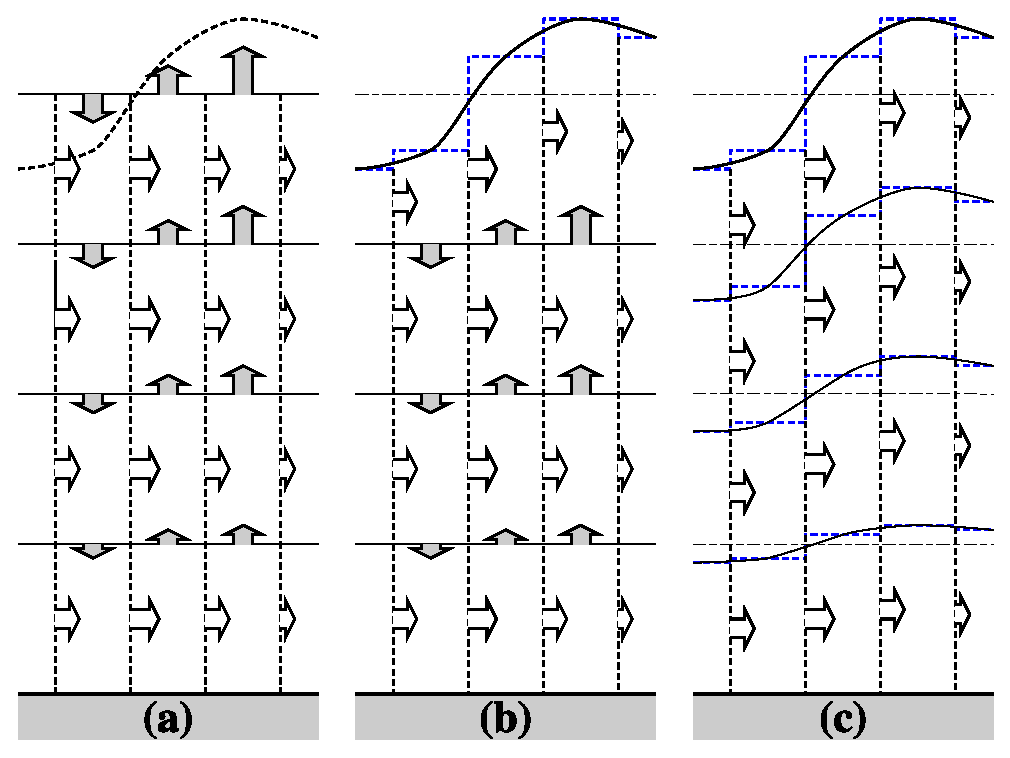
\includegraphics[width=0.66\textwidth]{MB_z_zstar}
  \caption[Curvilinear z-coordinate systems (\{non-\}linear free-surface cases and re-scaled \zstar)]{
    \begin{enumerate*}[label=(\textit{\alph*})]
    \item $z$-coordinate in linear free-surface case;
    \item $z$-coordinate in non-linear free surface case;
    \item re-scaled height coordinate
      (become popular as the \zstar-coordinate \citep{adcroft.campin_OM04}).
    \end{enumerate*}
  }
  \label{fig:MB_z_zstar}
\end{figure}

In this case, the free surface equation is nonlinear,
and the variations of volume are fully taken into account.
These coordinates systems is presented in a report \citep{levier.treguier.ea_trpt07} available on
the \NEMO\ web site.

The \zstar\ coordinate approach is an unapproximated, non-linear free surface implementation which
allows one to deal with large amplitude free-surface variations relative to the vertical resolution
\citep{adcroft.campin_OM04}.
In the \zstar\ formulation, the variation of the column thickness due to sea-surface undulations is
not concentrated in the surface level, as in the $z$-coordinate formulation,
but is equally distributed over the full water column.
Thus vertical levels naturally follow sea-surface variations, with a linear attenuation with depth,
as illustrated by \autoref{fig:MB_z_zstar}.
Note that with a flat bottom, such as in \autoref{fig:MB_z_zstar},
the bottom-following $z$ coordinate and \zstar\ are equivalent.
The definition and modified oceanic equations for the rescaled vertical coordinate \zstar,
including the treatment of fresh-water flux at the surface, are detailed in Adcroft and Campin (2004).
The major points are summarized here.
The position (\zstar) and vertical discretization ($\delta \zstar$) are expressed as:
\[
  % \label{eq:MB_z-star}
  H + \zstar = (H + z)  / r \quad \text{and}  \quad \delta \zstar = \delta z / r \quad \text{with} \quad r = \frac{H + \eta}{H}
\]
Simple re-organisation of the above expressions gives
\[
  % \label{eq:MB_zstar_2}
  \zstar = H \lt( \frac{z - \eta}{H + \eta} \rt)
\]
Since the vertical displacement of the free surface is incorporated in the vertical coordinate \zstar,
the upper and lower boundaries are at fixed \zstar\ position,
$\zstar = 0$ and $\zstar = -H$ respectively.
Also the divergence of the flow field is no longer zero as shown by the continuity equation:
\[
  \pd[r]{t} = \nabla_{\zstar} \cdot \lt( r \; \vect U_h \rt) + \pd[r \; w^*]{\zstar} = 0
\]
This \zstar\ coordinate is closely related to the $\eta$ coordinate used in many atmospheric models
(see Black (1994) for a review of $\eta$ coordinate atmospheric models).
It was originally used in ocean models by Stacey et al. (1995) for studies of tides next to shelves,
and it has been recently promoted by Adcroft and Campin (2004) for global climate modelling.

The surfaces of constant \zstar\ are quasi-horizontal.
Indeed, the \zstar\ coordinate reduces to $z$ when $\eta$ is zero.
In general, when noting the large differences between
undulations of the bottom topography versus undulations in the surface height,
it is clear that surfaces constant \zstar\ are very similar to the depth surfaces.
These properties greatly reduce difficulties of computing the horizontal pressure gradient relative to
terrain following sigma models discussed in \autoref{subsec:MB_sco}.
Additionally, since $\zstar = z$ when $\eta = 0$,
no flow is spontaneously generated in an unforced ocean starting from rest,
regardless the bottom topography.
This behaviour is in contrast to the case with ``s''-models,
where pressure gradient errors in the presence of nontrivial topographic variations can generate
nontrivial spontaneous flow from a resting state,
depending on the sophistication of the pressure gradient solver.
The quasi-horizontal nature of the coordinate surfaces also facilitates the implementation of
neutral physics parameterizations in \zstar\ models using the same techniques as in $z$-models
(see Chapters 13-16 of \cite{griffies_bk04}) for a discussion of neutral physics in $z$-models,
as well as \autoref{sec:LDF_slp} in this document for treatment in \NEMO).

The range over which \zstar\ varies is time independent $-H \leq \zstar \leq 0$.
Hence, all cells remain nonvanishing, so long as the surface height maintains $\eta > -H$.
This is a minor constraint relative to that encountered on the surface height when
using $s = z$ or $s = z - \eta$.

Because \zstar\ has a time independent range, all grid cells have static increments ds,
and the sum of the vertical increments yields the time independent ocean depth. %k ds = H.
The \zstar\ coordinate is therefore invisible to undulations of the free surface,
since it moves along with the free surface.
This property means that no spurious vertical transport is induced across
surfaces of constant \zstar\  by the motion of external gravity waves.
Such spurious transport can be a problem in z-models, especially those with tidal forcing.
Quite generally,
the time independent range for the \zstar\ coordinate is a very convenient property that
allows for a nearly arbitrary vertical resolution even in
the presence of large amplitude fluctuations of the surface height, again so long as $\eta > -H$.
%end MOM doc %%%

%% =================================================================================================
\subsection{Curvilinear terrain-following \textit{s}--coordinate}
\label{subsec:MB_sco}

Several important aspects of the ocean circulation are influenced by bottom topography.
Of course, the most important is that bottom topography determines deep ocean sub-basins, barriers,
sills and channels that strongly constrain the path of water masses, but more subtle effects exist.
For example,
the topographic $\beta$-effect is usually larger than the planetary one along continental slopes.
Topographic Rossby waves can be excited and can interact with the mean current.
In the $z$-coordinate system presented in the previous section (\autoref{sec:MB_zco}),
$z$-surfaces are geopotential surfaces.
The bottom topography is discretised by steps.
This often leads to a misrepresentation of a gradually sloping bottom and to
large localized depth gradients associated with large localized vertical velocities.
The response to such a velocity field often leads to numerical dispersion effects.
One solution to strongly reduce this error is to use a partial step representation of
bottom topography instead of a full step one \cite{pacanowski.gnanadesikan_MWR98}.
Another solution is to introduce a terrain-following coordinate system (hereafter $s$-coordinate).

The $s$-coordinate avoids the discretisation error in the depth field since
the layers of computation are gradually adjusted with depth to the ocean bottom.
Relatively small topographic features as well as
gentle, large-scale slopes of the sea floor in the deep ocean,
which would be ignored in typical $z$-model applications with
the largest grid spacing at greatest depths,
can easily be represented (with relatively low vertical resolution).
A terrain-following model (hereafter $s$-model) also facilitates
the modelling of the boundary layer flows over a large depth range,
which in the framework of the $z$-model would require high vertical resolution over
the whole depth range.
Moreover,
with a $s$-coordinate it is possible, at least in principle, to have the bottom and the sea surface as
the only boundaries of the domain (no more lateral boundary condition to specify).
Nevertheless, a $s$-coordinate also has its drawbacks.
Perfectly adapted to a homogeneous ocean,
it has strong limitations as soon as stratification is introduced.
The main two problems come from the truncation error in the horizontal pressure gradient and
a possibly increased diapycnal diffusion.
The horizontal pressure force in $s$-coordinate consists of two terms (see \autoref{apdx:SCOORD}),
\begin{equation}
  \label{eq:MB_p_sco}
  \nabla p |_z = \nabla p |_s - \frac{1}{e_3} \pd[p]{s} \nabla z |_s
\end{equation}

The second term in \autoref{eq:MB_p_sco} depends on the tilt of the coordinate surface and
leads to a truncation error that is not present in a $z$-model.
In the special case of a $\sigma$-coordinate
(i.e. a depth-normalised coordinate system $\sigma = z/H$),
\citet{haney_JPO91} and \citet{beckmann.haidvogel_JPO93} have given estimates of
the magnitude of this truncation error.
It depends on topographic slope, stratification, horizontal and vertical resolution,
the equation of state, and the finite difference scheme.
This error limits the possible topographic slopes that a model can handle at
a given horizontal and vertical resolution.
This is a severe restriction for large-scale applications using realistic bottom topography.
The large-scale slopes require high horizontal resolution,
and the computational cost becomes prohibitive.
This problem can be at least partially overcome by mixing $s$-coordinate and
step-like representation of bottom topography
\citep{gerdes_JGR93,gerdes_JGR93*a,madec.delecluse.ea_JPO96}.
However, the definition of the model domain vertical coordinate becomes then a non-trivial thing for
a realistic bottom topography:
an envelope topography is defined in $s$-coordinate on which
a full or partial step bottom topography is then applied in order to
adjust the model depth to the observed one (see \autoref{subsec:DOM_zgr}).

For numerical reasons a minimum of diffusion is required along
the coordinate surfaces of any finite difference model.
It causes spurious diapycnal mixing when coordinate surfaces do not coincide with isoneutral surfaces.
This is the case for a $z$-model as well as for a $s$-model.
However, density varies more strongly on $s$-surfaces than on horizontal surfaces in
regions of large topographic slopes,
implying larger diapycnal diffusion in a $s$-model than in a $z$-model.
Whereas such a diapycnal diffusion in a $z$-model tends to
weaken horizontal density (pressure) gradients and thus the horizontal circulation,
it usually reinforces these gradients in a $s$-model, creating spurious circulation.
For example, imagine an isolated bump of topography in
an ocean at rest with a horizontally uniform stratification.
Spurious diffusion along $s$-surfaces will induce a bump of isoneutral surfaces over the topography,
and thus will generate there a baroclinic eddy.
In contrast, the ocean will stay at rest in a $z$-model.
As for the truncation error, the problem can be reduced by
introducing the terrain-following coordinate below the strongly stratified portion of the water column
(\ie\ the main thermocline) \citep{madec.delecluse.ea_JPO96}.
An alternate solution consists of rotating the lateral diffusive tensor to
geopotential or to isoneutral surfaces (see \autoref{subsec:MB_ldf}).
Unfortunately, the slope of isoneutral surfaces relative to the $s$-surfaces can very large,
strongly exceeding the stability limit of such a operator when it is discretized
(see \autoref{chap:LDF}).

The $s$-coordinates introduced here \citep{lott.madec.ea_OM90,madec.delecluse.ea_JPO96}
differ mainly in two aspects from similar models:
it allows a representation of bottom topography with
mixed full or partial step-like/terrain following topography;
It also offers a completely general transformation, $s=s(i,j,z)$ for the vertical coordinate.

%% =================================================================================================
\subsection{Curvilinear \ztilde-coordinate}
\label{subsec:MB_zco_tilde}

The \ztilde-coordinate has been developed by \citet{leclair.madec_OM11}.
It is available in \NEMO\ since the version 3.4 and is more robust in version 4.0 than previously.
Nevertheless, it is currently not robust enough to be used in all possible configurations.
Its use is therefore not recommended.

%% =================================================================================================
\section{Subgrid scale physics}
\label{sec:MB_zdf_ldf}

The hydrostatic primitive equations describe the behaviour of a geophysical fluid at
space and time scales larger than a few kilometres in the horizontal,
a few meters in the vertical and a few minutes.
They are usually solved at larger scales: the specified grid spacing and time step of
the numerical model.
The effects of smaller scale motions (coming from the advective terms in the Navier-Stokes equations)
must be represented entirely in terms of large-scale patterns to close the equations.
These effects appear in the equations as the divergence of turbulent fluxes
(\ie\ fluxes associated with the mean correlation of small scale perturbations).
Assuming a turbulent closure hypothesis is equivalent to choose a formulation for these fluxes.
It is usually called the subgrid scale physics.
It must be emphasized that this is the weakest part of the primitive equations,
but also one of the most important for long-term simulations as
small scale processes \textit{in fine} balance the surface input of kinetic energy and heat.

The control exerted by gravity on the flow induces a strong anisotropy between
the lateral and vertical motions.
Therefore subgrid-scale physics \textbf{D}$^{\vect U}$, $D^{S}$ and $D^{T}$  in
\autoref{eq:MB_PE_dyn}, \autoref{eq:MB_PE_tra_T} and \autoref{eq:MB_PE_tra_S} are divided into
a  lateral part \textbf{D}$^{l \vect U}$, $D^{l S}$ and $D^{l T}$ and
a vertical part \textbf{D}$^{v \vect U}$, $D^{v S}$ and $D^{v T}$.
The formulation of these terms and their underlying physics are briefly discussed in
the next two subsections.

%% =================================================================================================
\subsection{Vertical subgrid scale physics}
\label{subsec:MB_zdf}

The model resolution is always larger than the scale at which
the major sources of vertical turbulence occur (shear instability, internal wave breaking...).
Turbulent motions are thus never explicitly solved, even partially, but always parameterized.
The vertical turbulent fluxes are assumed to depend linearly on
the gradients of large-scale quantities (for example,
the turbulent heat flux is given by $\overline{T' w'} = -A^{v T} \partial_z \overline T$,
where $A^{v T}$ is an eddy coefficient).
This formulation is analogous to that of molecular diffusion and dissipation.
This is quite clearly a necessary compromise: considering only the molecular viscosity acting on
large scale severely underestimates the role of turbulent diffusion and dissipation,
while an accurate consideration of the details of turbulent motions is simply impractical.
The resulting vertical momentum and tracer diffusive operators are of second order:
\begin{equation}
  \label{eq:MB_zdf}
  \begin{gathered}
    \vect D^{v \vect U} = \pd[]{z} \lt( A^{vm} \pd[\vect U_h]{z} \rt) \text{,} \
          D^{vT}       = \pd[]{z} \lt( A^{vT} \pd[T]{z}         \rt) \ \text{and} \
          D^{vS}       = \pd[]{z} \lt( A^{vT} \pd[S]{z}         \rt)
  \end{gathered}
\end{equation}
where $A^{vm}$ and $A^{vT}$ are the vertical eddy viscosity and diffusivity coefficients,
respectively.
At the sea surface and at the bottom, turbulent fluxes of momentum, heat and salt must be specified
(see \autoref{chap:SBC} and \autoref{chap:ZDF} and \autoref{sec:TRA_bbl}).
All the vertical physics is embedded in the specification of the eddy coefficients.
They can be assumed to be either constant, or function of the local fluid properties
(\eg\ Richardson number, Brunt-V\"{a}is\"{a}l\"{a} frequency, distance from the boundary ...),
or computed from a turbulent closure model.
The choices available in \NEMO\ are discussed in \autoref{chap:ZDF}).

%% =================================================================================================
\subsection{Formulation of the lateral diffusive and viscous operators}
\label{subsec:MB_ldf}

Lateral turbulence can be roughly divided into a mesoscale turbulence associated with eddies
(which can be solved explicitly if the resolution is sufficient since
their underlying physics are included in the primitive equations),
and a sub mesoscale turbulence which is never explicitly solved even partially,
but always parameterized.
The formulation of lateral eddy fluxes depends on whether
the mesoscale is below or above the grid-spacing (\ie\ the model is eddy-resolving or not).

In non-eddy-resolving configurations, the closure is similar to that used for the vertical physics.
The lateral turbulent fluxes are assumed to depend linearly on
the lateral gradients of large-scale quantities.
The resulting lateral diffusive and dissipative operators are of second order.
Observations show that
lateral mixing induced by mesoscale turbulence tends to be along isopycnal surfaces
(or more precisely neutral surfaces \cite{mcdougall_JPO87}) rather than across them.
As the slope of neutral surfaces is small in the ocean,
a common approximation is to assume that the ``lateral'' direction is the horizontal,
\ie\ the lateral mixing is performed along geopotential surfaces.
This leads to a geopotential second order operator for lateral subgrid scale physics.
This assumption can be relaxed:
the eddy-induced turbulent fluxes can be better approached by assuming that
they depend linearly on the gradients of large-scale quantities computed along neutral surfaces.
In such a case, the diffusive operator is an isoneutral second order operator and
it has components in the three space directions.
However, both horizontal and isoneutral operators have no effect on
mean (\ie\ large scale) potential energy whereas
potential energy is a main source of turbulence (through baroclinic instabilities).
\citet{gent.mcwilliams_JPO90} proposed a parameterisation of mesoscale eddy-induced turbulence which
associates an eddy-induced velocity to the isoneutral diffusion.
Its mean effect is to reduce the mean potential energy of the ocean.
This leads to a formulation of lateral subgrid-scale physics made up of
an isoneutral second order operator and an eddy induced advective part.
In all these lateral diffusive formulations,
the specification of the lateral eddy coefficients remains the problematic point as
there is no really satisfactory formulation of these coefficients as
a function of large-scale features.

In eddy-resolving configurations, a second order operator can be used,
but usually the more scale selective biharmonic operator is preferred as
the grid-spacing is usually not small enough compared to the scale of the eddies.
The role devoted to the subgrid-scale physics is to dissipate the energy that
cascades toward the grid scale and thus to ensure the stability of the model while
not interfering with the resolved mesoscale activity.
Another approach is becoming more and more popular:
instead of specifying explicitly a sub-grid scale term in
the momentum and tracer time evolution equations,
one uses an advective scheme which is diffusive enough to maintain the model stability.
It must be emphasised that then,
all the sub-grid scale physics is included in the formulation of the advection scheme.

All these parameterisations of subgrid scale physics have advantages and drawbacks.
They are not all available in \NEMO.
For active tracers (temperature and salinity) the main ones are:
Laplacian and bilaplacian operators acting along geopotential or iso-neutral surfaces,
\citet{gent.mcwilliams_JPO90} parameterisation, and various slightly diffusive advection schemes.
For momentum, the main ones are:
Laplacian and bilaplacian operators acting along geopotential surfaces,
and UBS advection schemes when flux form is chosen for the momentum advection.

%% =================================================================================================
\subsubsection{Lateral laplacian tracer diffusive operator}

The lateral Laplacian tracer diffusive operator is defined by (see \autoref{apdx:DIFFOPERS}):
\begin{equation}
  \label{eq:MB_iso_tensor}
  D^{lT} = \nabla \vect . \lt( A^{lT} \; \Re \; \nabla T \rt) \quad \text{with} \quad \Re =
  \begin{pmatrix}
    1    & 0    & -r_1          \\
    0    & 1    & -r_2          \\
    -r_1 & -r_2 & r_1^2 + r_2^2 \\
  \end{pmatrix}
\end{equation}
where $r_1$ and $r_2$ are the slopes between the surface along which the diffusive operator acts and
the model level (\eg\ $z$- or $s$-surfaces).
Note that the formulation \autoref{eq:MB_iso_tensor} is exact for
the rotation between geopotential and $s$-surfaces,
while it is only an approximation for the rotation between isoneutral and $z$- or $s$-surfaces.
Indeed, in the latter case, two assumptions are made to simplify \autoref{eq:MB_iso_tensor}
\citep{cox_OM87}.
First, the horizontal contribution of the dianeutral mixing is neglected since
the ratio between iso and dia-neutral diffusive coefficients is known to be
several orders of magnitude smaller than unity.
Second, the two isoneutral directions of diffusion are assumed to be independent since
the slopes are generally less than $10^{-2}$ in the ocean (see \autoref{apdx:DIFFOPERS}).

For \textit{iso-level} diffusion, $r_1$ and $r_2 $ are zero.
$\Re$ reduces to the identity in the horizontal direction, no rotation is applied.

For \textit{geopotential} diffusion,
$r_1$ and $r_2 $ are the slopes between the geopotential and computational surfaces:
they are equal to $\sigma_1$ and $\sigma_2$, respectively (see \autoref{eq:MB_sco_slope}).

For \textit{isoneutral} diffusion $r_1$ and $r_2$ are the slopes between
the isoneutral and computational surfaces.
Therefore, they are different quantities, but have similar expressions in $z$- and $s$-coordinates.
In $z$-coordinates:
\begin{equation}
  \label{eq:MB_iso_slopes}
  r_1 = \frac{e_3}{e_1} \lt( \pd[\rho]{i} \rt) \lt( \pd[\rho]{k} \rt)^{-1} \quad
  r_2 = \frac{e_3}{e_2} \lt( \pd[\rho]{j} \rt) \lt( \pd[\rho]{k} \rt)^{-1}
\end{equation}
while in $s$-coordinates $\pd[]{k}$ is replaced by $\pd[]{s}$.

%% =================================================================================================
\subsubsection{Eddy induced velocity}

When the \textit{eddy induced velocity} parametrisation (eiv) \citep{gent.mcwilliams_JPO90} is used,
an additional tracer advection is introduced in combination with the isoneutral diffusion of tracers:
\[
  % \label{eq:MB_iso+eiv}
  D^{lT} = \nabla \cdot \lt( A^{lT} \; \Re \; \nabla T \rt) + \nabla \cdot \lt( \vect U^\ast \, T \rt)
\]
where $ \vect U^\ast = \lt( u^\ast,v^\ast,w^\ast \rt)$ is a non-divergent,
eddy-induced transport velocity. This velocity field is defined by:
\[
  % \label{eq:MB_eiv}
  u^\ast =   \frac{1}{e_3}            \pd[]{k} \lt( A^{eiv} \;        \tilde{r}_1 \rt) \quad
  v^\ast =   \frac{1}{e_3}            \pd[]{k} \lt( A^{eiv} \;        \tilde{r}_2 \rt) \quad
  w^\ast = - \frac{1}{e_1 e_2} \lt[   \pd[]{i} \lt( A^{eiv} \; e_2 \, \tilde{r}_1 \rt)
                                     + \pd[]{j} \lt( A^{eiv} \; e_1 \, \tilde{r}_2 \rt) \rt]
\]
where $A^{eiv}$ is the eddy induced velocity coefficient
(or equivalently the isoneutral thickness diffusivity coefficient),
and $\tilde r_1$ and $\tilde r_2$ are the slopes between
isoneutral and \textit{geopotential} surfaces.
Their values are thus independent of the vertical coordinate,
but their expression depends on the coordinate:
\begin{equation}
  \label{eq:MB_slopes_eiv}
  \tilde{r}_n =
    \begin{cases}
      r_n            & \text{in $z$-coordinate}                \\
      r_n + \sigma_n & \text{in \zstar- and $s$-coordinates}
    \end{cases}
  \quad \text{where~} n = 1, 2
\end{equation}

The normal component of the eddy induced velocity is zero at all the boundaries.
This can be achieved in a model by tapering either the eddy coefficient or the slopes to zero in
the vicinity of the boundaries.
The latter strategy is used in \NEMO\ (cf. \autoref{chap:LDF}).

%% =================================================================================================
\subsubsection{Lateral bilaplacian tracer diffusive operator}

The lateral bilaplacian tracer diffusive operator is defined by:
\[
  % \label{eq:MB_bilapT}
  D^{lT}= - \Delta \; (\Delta T) \quad \text{where} \quad
  \Delta \bullet = \nabla \lt( \sqrt{B^{lT}} \; \Re \; \nabla \bullet \rt)
\]
It is the Laplacian operator given by \autoref{eq:MB_iso_tensor} applied twice with
the harmonic eddy diffusion coefficient set to the square root of the biharmonic one.

%% =================================================================================================
\subsubsection{Lateral Laplacian momentum diffusive operator}

The Laplacian momentum diffusive operator along $z$- or $s$-surfaces is found by
applying \autoref{eq:MB_lap_vector} to the horizontal velocity vector (see \autoref{apdx:DIFFOPERS}):
\begin{align*}
  % \label{eq:MB_lapU}
  \vect D^{l \vect U} &=   \nabla_h        \big( A^{lm}    \chi             \big)
                         - \nabla_h \times \big( A^{lm} \, \zeta \; \vect k \big) \\
                      &= \lt(   \frac{1}{e_1}     \pd[ \lt( A^{lm}    \chi      \rt) ]{i} \rt.
                              - \frac{1}{e_2 e_3} \pd[ \lt( A^{lm} \; e_3 \zeta \rt) ]{j} ,
                                \frac{1}{e_2}     \pd[ \lt( A^{lm}    \chi      \rt) ]{j}
                         \lt. + \frac{1}{e_1 e_3} \pd[ \lt( A^{lm} \; e_3 \zeta \rt) ]{i} \rt)
\end{align*}

Such a formulation ensures a complete separation between
the vorticity and horizontal divergence fields (see \autoref{apdx:INVARIANTS}).
Unfortunately, it is only available in \textit{iso-level} direction.
When a rotation is required
(\ie\ geopotential diffusion in $s$-coordinates or
isoneutral diffusion in both $z$- and $s$-coordinates),
the $u$ and $v$-fields are considered as independent scalar fields,
so that the diffusive operator is given by:
\[
  % \label{eq:MB_lapU_iso}
    D_u^{l \vect U} = \nabla . \lt( A^{lm} \; \Re \; \nabla u \rt) \quad
    D_v^{l \vect U} = \nabla . \lt( A^{lm} \; \Re \; \nabla v \rt)
\]
where $\Re$ is given by \autoref{eq:MB_iso_tensor}.
It is the same expression as those used for diffusive operator on tracers.
It must be emphasised that such a formulation is only exact in a Cartesian coordinate system,
\ie\ on a $f$- or $\beta$-plane, not on the sphere.
It is also a very good approximation in vicinity of the Equator in
a geographical coordinate system \citep{lengaigne.madec.ea_JGR03}.

%% =================================================================================================
\subsubsection{Lateral bilaplacian momentum diffusive operator}

As for tracers,
the bilaplacian order momentum diffusive operator is a re-entering Laplacian operator with
the harmonic eddy diffusion coefficient set to the square root of the biharmonic one.
Nevertheless it is currently not available in the iso-neutral case.

\subinc{%% =================================================================================================
%% Backmatter
%% =================================================================================================

%% Bibliography
%% =================================================================================================

\phantomsection
\addcontentsline{toc}{chapter}{Bibliography}
\lohead{Bibliography}
\rehead{Bibliography}
\bibliography{../main/bibliography}

\clearpage

%% Indices
%% =================================================================================================

\phantomsection
\addcontentsline{toc}{chapter}{Indices}
\lohead{Indices}
\rehead{Indices}
\printindex[blocks]
\printindex[keys]
\printindex[modules]
\printindex[parameters]
\printindex[subroutines]

\clearpage

%% Glossary
%% =================================================================================================

%\phantomsection
%\addcontentsline{toc}{chapter}{Glossary}
%\lohead{Glossary}\rehead{Glossary}
%\printglossaries
}

\end{document}
